\chapter{Challenges and Contributions}

\label{ch:summary}

This chapter gives an overall idea of the challenges faced during the development process and the ways they were handled to sort the issues and overcome them with a workaround or a different possible solution. Also, the application highlights some of the future woks which can make the application to a successful product in the market.

\section{Challenges Faced}
The developer has undergone various challenges during the development of the application which includes the ground research and understanding of the application and core study process to develop the initial prototype. Though there were some challenges the developer successfully overcame most of them and able to develop the working model with sufficient guidance from supervisors. 
Here are some of the explicit challenges faced during the whole process:
\begin{itemize}
    \item Selecting the right \textbf{news dataset} was the foremost challenge as the news content is the primary importance for the application. The news dataset comes with the image, image url, source information, description and title, etc.
    The news dataset was then taken from the Newsapi service which provides api json response from various sources and countries. 
    
    \item \textbf{Personalization} is one of the most interested feature for any web applications and it required ground research and complex study to understand how well it can be made to this application. After reviewing many research papers and understanding existing applications, the developer was able to collaborate many views of personalization into this application.
    
    \item Developing the\textbf{ front end components} from scratch in a user-friendly manner was bit time consuming for the project to decide on the layout and the wireframe diagrams.
    
    \item The other viewpoint of projections required brief study on how different kinds of charts work with angular and support of interactive map libraries. After analysing D3, leaflet, finally \textbf{amcharts} has been chosen as it has support for many charts and also geographical map projects with sufficient documentation for understanding. 
    
    \item Updating category and country filter at the same time was bit tricky to keep in memory the old selection of one while the other changes to list the appropriate results. This was resolved with the usage of Behavioral subject which effectively resolved this issue.
    
    \item \textbf{JWT authentication} is a key mechanism to control login and token management and allows secured access to the functions. This was initially hard to understand and bit complex but resolved over time.
    
    \item The system needs to manage each user with own preferred news and weight based on their interests as a part of user profiling which was challenging to accomplish with a hashmap. The development of logical algorithm for the programming and making sure it works as expected was complex to achieve and required to note very minute details in updating the user behaviour everytime.
    
    \item Finally Recommendation system required major research on various existing applications and better way to recommend news articles with machine learning algorithm. This puzzle was successfully resolved using Mahout recommendation system which has very good java implementation support.
    
\end{itemize}


\section{Results Achieved}
The application called 'Personalized Buzzfeed' works as expected and is observed and tested for the successful achievement of its main objectives. 
The application provides the news articles for all the users and once the user logs in, it takes the user interactions and presents the user's personalized news articles which is worked out in background by personalization algorithm called weight-map algorithm.
These are the general and personalized news feed in the front-end.
 \begin{figure}[h!]
    \begin{multicols}{2}
    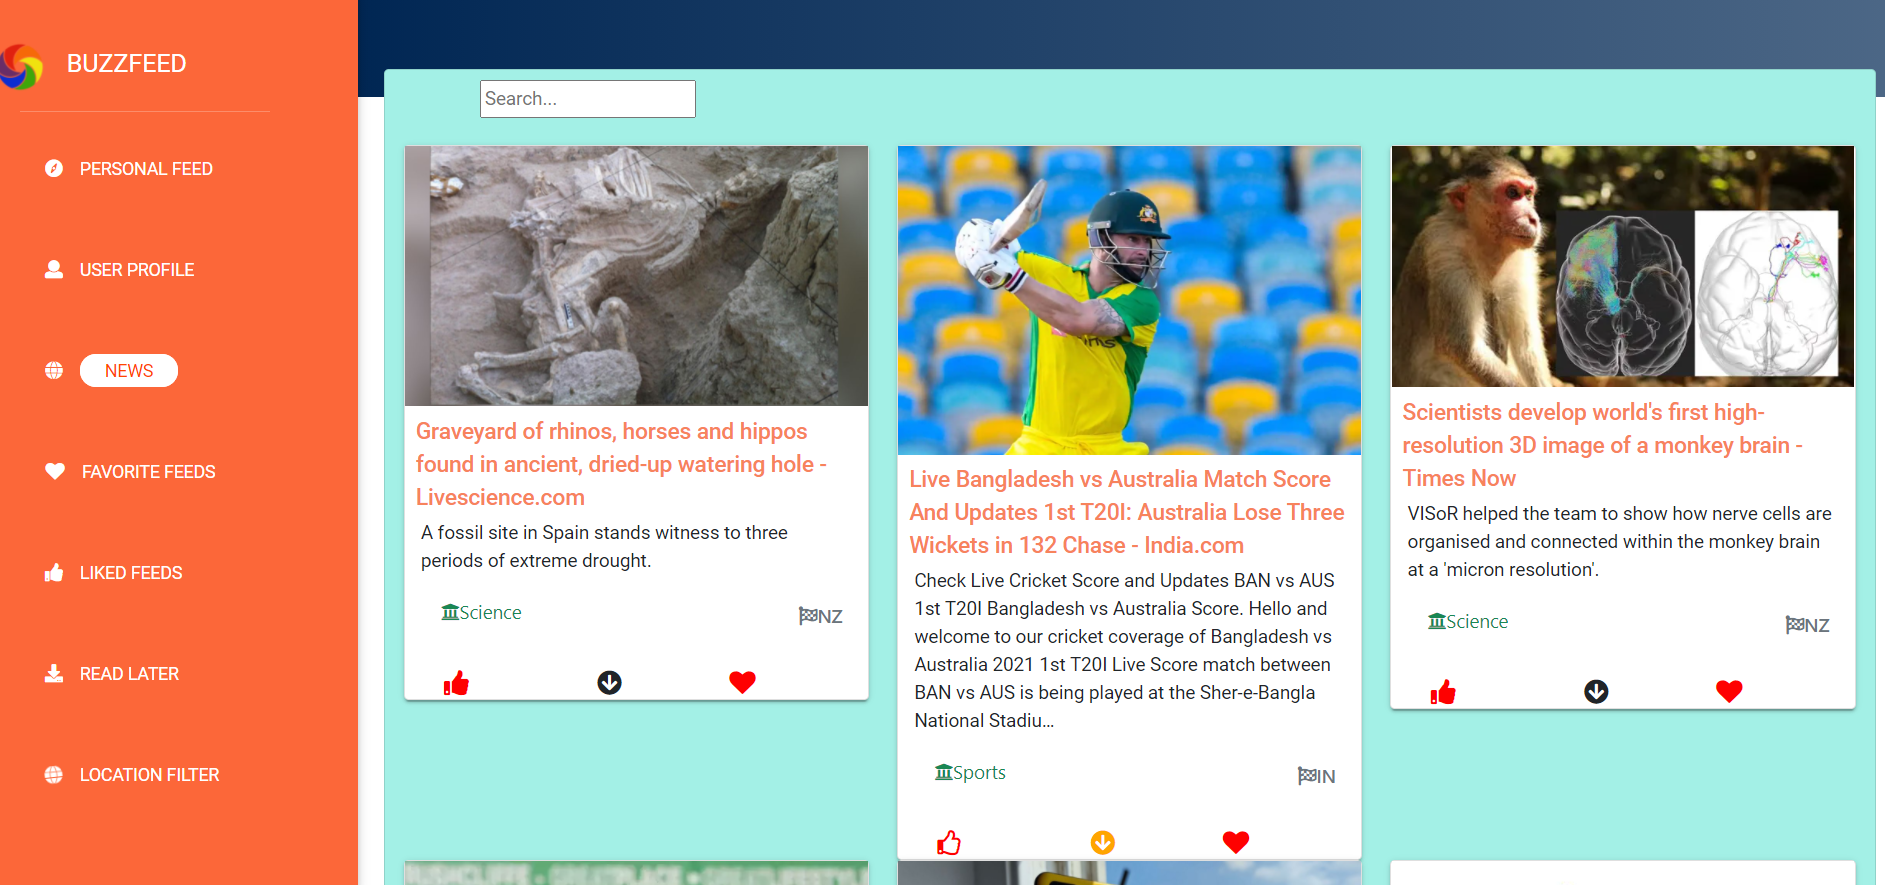
\includegraphics[width=\linewidth]{images/NewsFeed.PNG}\par 
    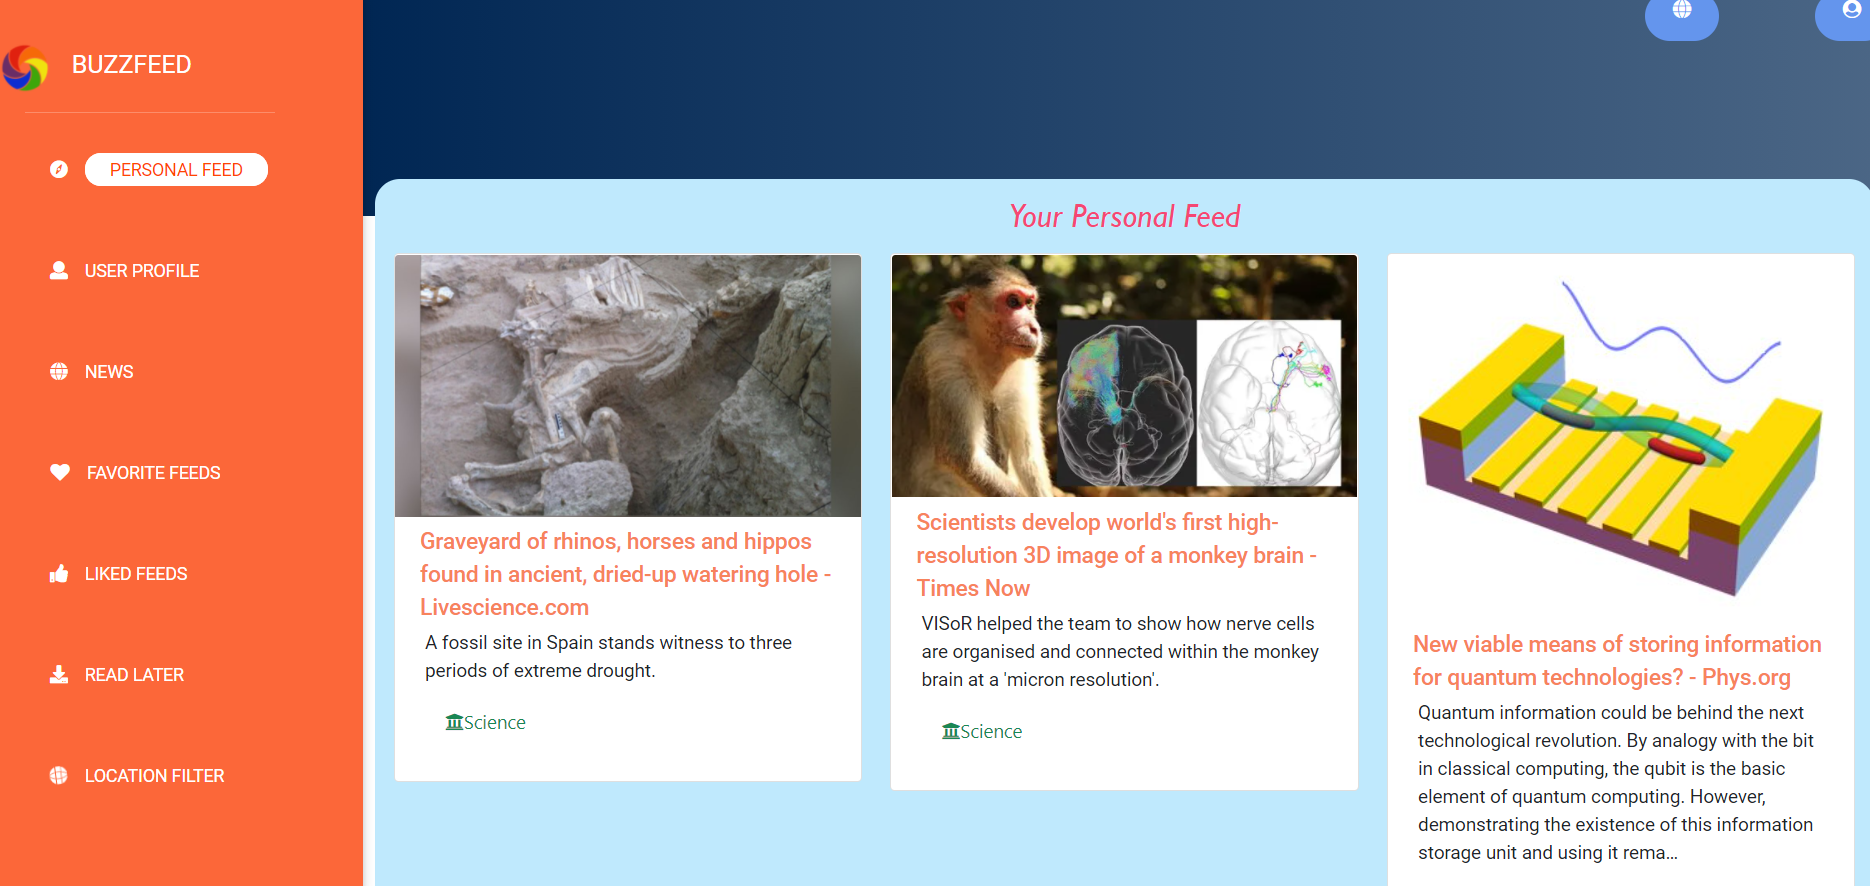
\includegraphics[width=\linewidth]{images/userFeed.PNG}\par 
    \end{multicols}

\centering \caption{Personalization}
\end{figure}

Visualization is presented in two major areas by amcharts which makes it interactive and more clear for understanding.
Below are the user charts projection and global map visualization in the front-end.
\begin{figure}[h!]
    \begin{multicols}{2}
    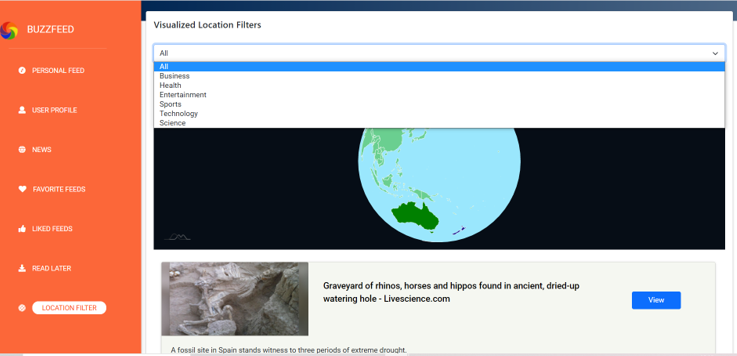
\includegraphics[width=\linewidth]{images/Locationfilter.PNG}\par 
    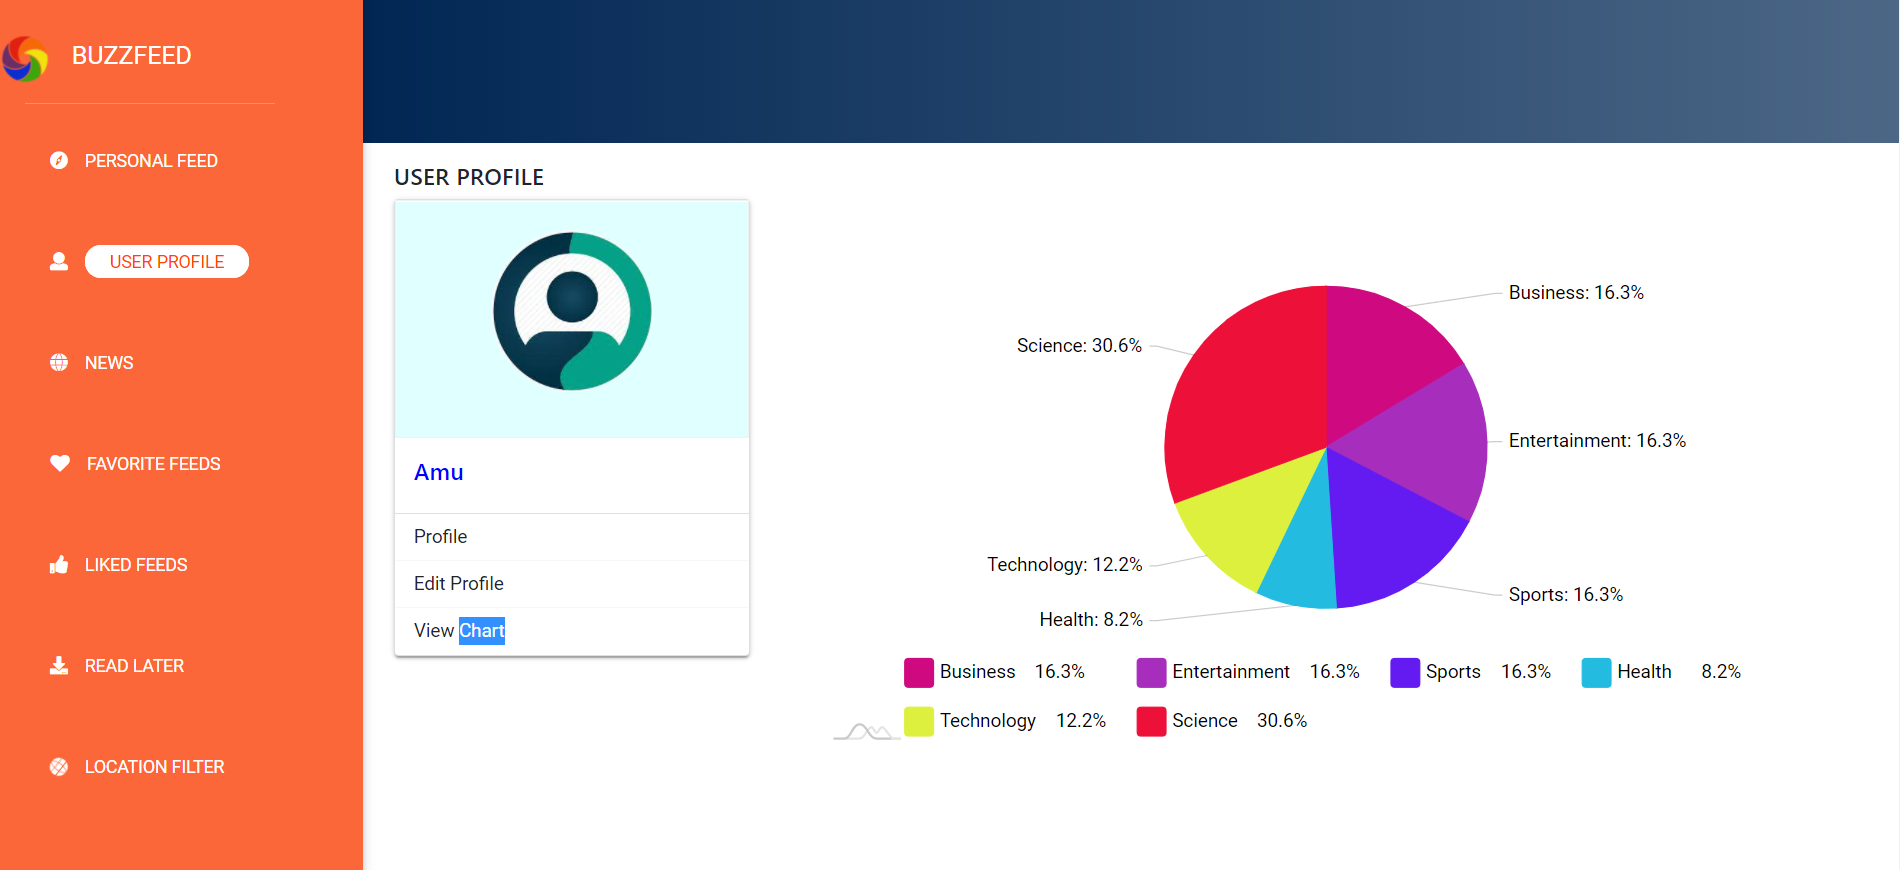
\includegraphics[width=\linewidth]{images/userchart.PNG}\par 
    \end{multicols}

\centering \caption{Visualization}
\end{figure}

Recommendation is achieved by Apache Mahout Recommendation machine learning algorithm and it appears in the client if the user similarity pattern is observed.
Here is a below example where the user-user similarity is observed and the application notifies the user.\newline

\begin{figure}[h!]
    \begin{center}
    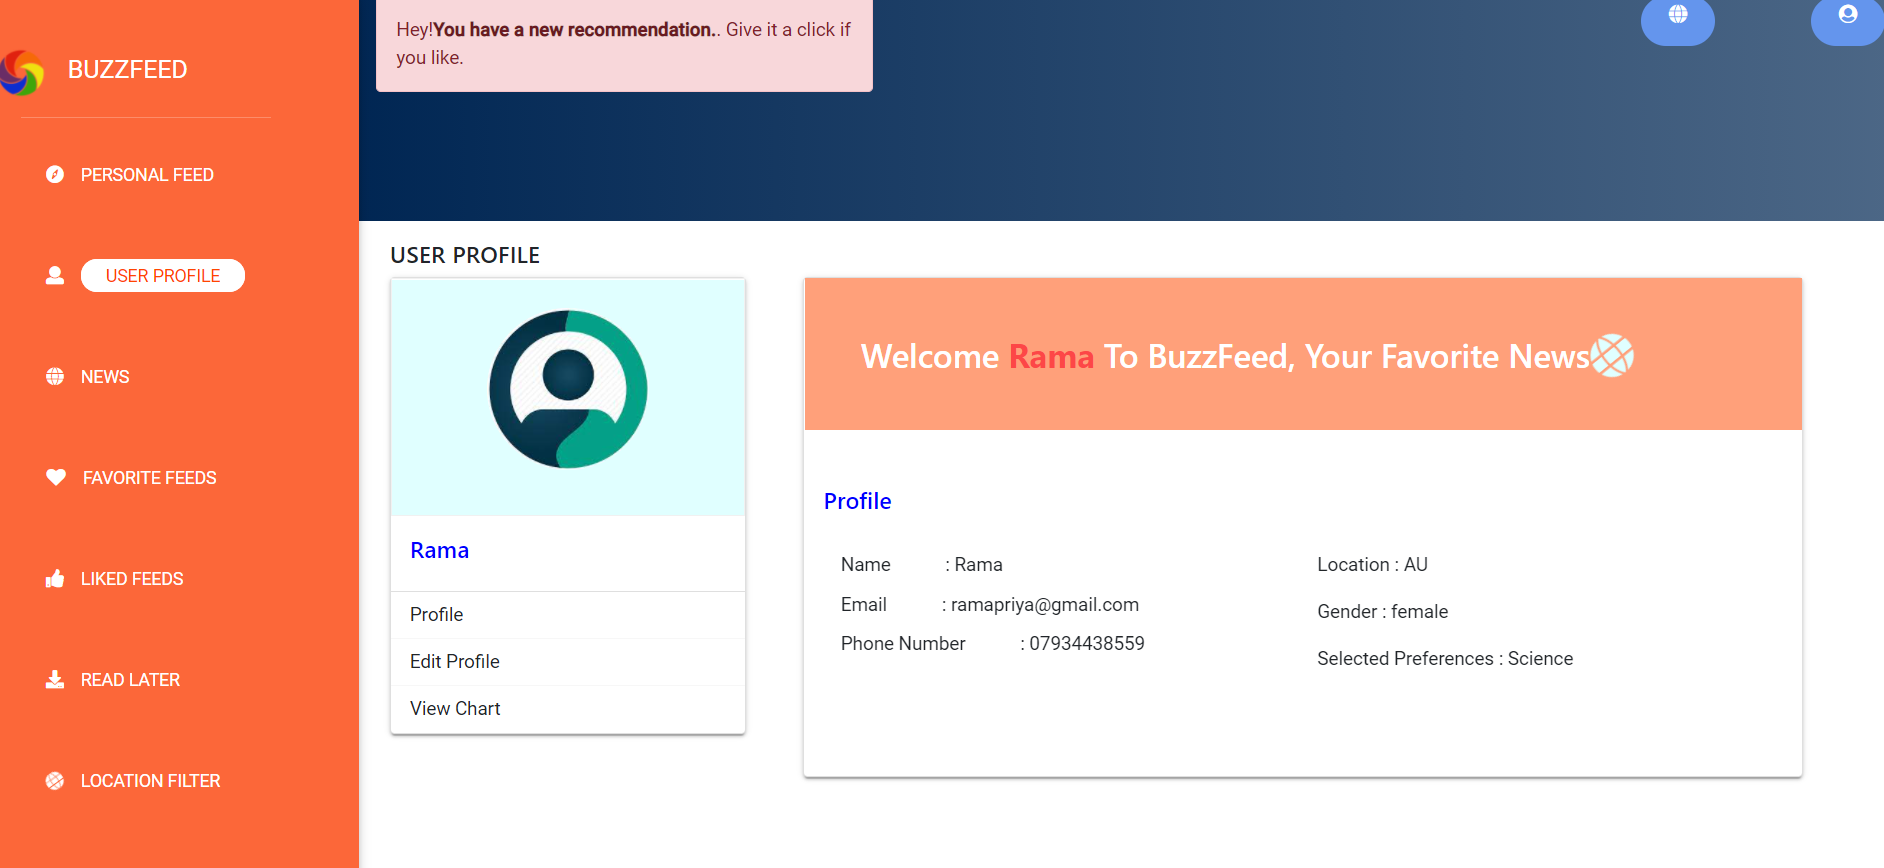
\includegraphics[width=\linewidth]{images/UserProfile_recommendation.PNG}\par
    \end{center}
\centering \caption{Recommendation}
\end{figure}


Evaluation is all done with Observation testing and Test Driven Development and fixed some of the bugs which popped up during the process and below are the successful testcases.


\section{Future Work}

The application developed right now resolves all major stakeholder requirements and successfully available as a working prototype which can be further enhanced and developed to deliver it as a product out in the market.
The possible enhancements could include some of the following.

\begin{itemize}
    \item Enhance projections and visualization to make it more interactive and user-friendly.
    \item News dataset could have been taken with some popularity field to understand how much trending the news is.
    \item Recommendation model can further include item-user correlation and added to current user-user similarity to understand similar categories which can be correlated like health can be interlinked nutrition and so on. For this the news dataset may be extended further with license to have majority of categories data from same or different third party APIs who support them.
    \item User profiling could be extended with options to track implicit user behavior and interests.
\end{itemize}


